\newpage
\section{Setting up the workspace}
\genHeader

Nowadays, \emph{no one} writes a complex parser completely by hand. Although this is sometimes still necessary for syntactically challenging languages, most
parsers can be quickly whipped up using context-free \emph{string grammars}.\footnote{For simple cases, \emph{regular expressions} can also be used} These are
typically written in Extended Backus-Naur Form (EBNF)\define{EBNF}. ANTLR~\cite{ANTLR} is a tool that can generate a parser from this compact specification for
a host of target programming languages, including Java. Although ANTLR might not be the most efficient or powerful parser generator, it is open-source, well
documented and supported, and allows for a pragmatic and elegant fallback to Java when things get nasty and we have to resort to some dirty tricks to get our
job done.

A parser, of course, is based on whatever model it must work with. Given that we want to parse to and from a dictionary, we need to have the
\texttt{DictionaryLanguage} metamodel defined before starting. The dictionary is a relatively simple device, so you have three options to loading this project
into your workspace:

% Options
\begin{description}
% -- Metamodel Screenshots ---
\item[Option 1:] You can start a new metamodel project called \texttt{Dictionary} (Fig.~\ref{eclipse:startMetamodel}) and complete a
\texttt{DictionaryLanguage} package until it matches either Fig.~\ref{ea:dictLang} or Fig.~\ref{eclipse:dictLang}.\footnote{Review metamodel construction by
working through Part II: Ecore}

\begin{figure}[htbp]
\begin{center}
  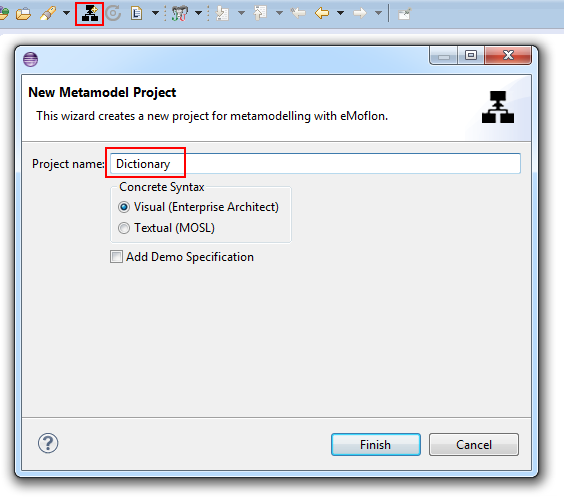
\includegraphics[width=0.65\textwidth]{eclipse_startDictionary}
  \caption{Begin parser project}
  \label{eclipse:startMetamodel}
\end{center}
\end{figure}

\newpage

\vspace*{1cm}

\begin{figure}[htb]
\begin{center}
  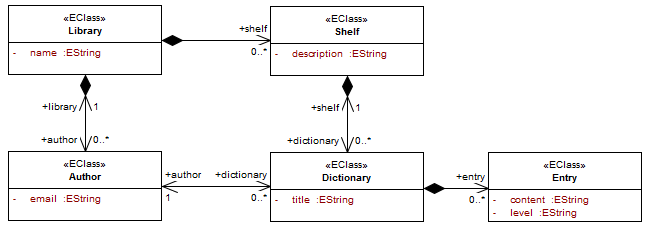
\includegraphics[width=\textwidth]{ea_dictionaryMetamodel}
  \caption{TCreate the package in \texttt{My Working Set} with an eMoflon Ecore diagram of the same name.}
  \label{ea:dictLang}
\end{center}
\end{figure}

\vspace{1cm}

\begin{figure}[htb]
\begin{center}
  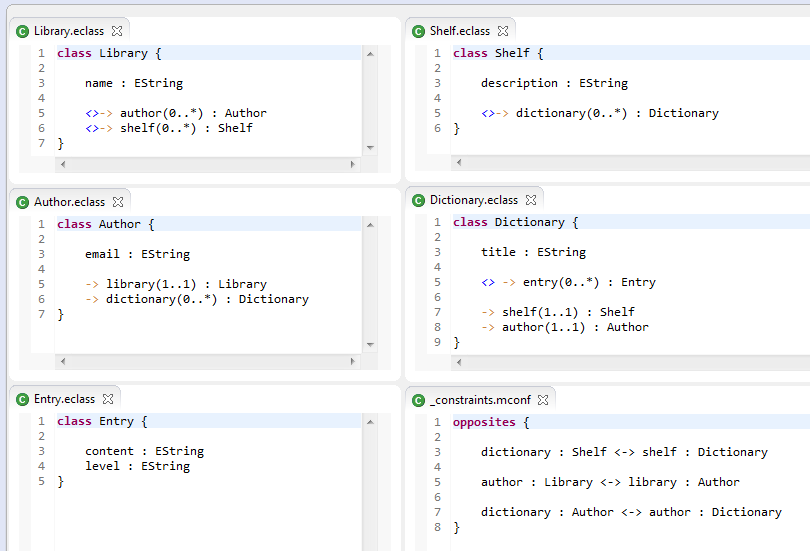
\includegraphics[width=0.8\textwidth]{eclipse_dictionaryMetamodel}
  \caption{\texttt{Dictionary} constructed in Eclipse \update}
  \label{eclipse:dictLang}
\end{center}
\end{figure}

\newpage

% -- Cheat Package(s)
\newpage
\item[Option 2:] You can download our cheat package and load \texttt{Dictionary} into your workspace using the Eclipse ``New" wizard
(Fig.~\ref{eclipse_cheatPackage}).

\vspace{0.5cm}

\begin{figure}[htbp]
\begin{center}
  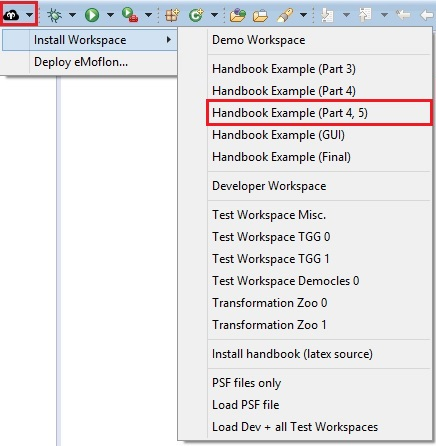
\includegraphics[width=0.65\textwidth]{eclipse_loadDictionaryProject}
  \caption{Load a \texttt{Dictionary} project into your workspace}
  \label{eclipse_cheatPackage}
\end{center}
\end{figure}

\item[$\blacktriangleright$] Pressing \texttt{Finish} will load either a MOSL directory or \texttt{DictionaryLanguage.eap} file into a working set, depending on
your syntax choice (Fig.~\ref{ea:cheatLoaded} or Fig.~\ref{eclipse:cheatLoaded}).

\begin{figure}[htbp]
   \centering
      \subfloat[comment 1 \update]{
        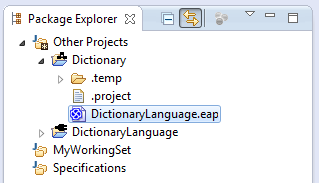
\includegraphics[width=0.45\textwidth]{eclipse_loadedCheatPackageVisual}
        \label{ea:cheatLoaded}
      }
      \subfloat[Bugger. Comment 2]{
        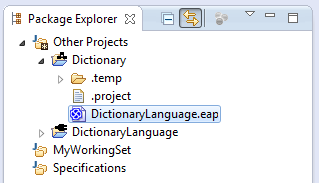
\includegraphics[width=0.45\textwidth]{eclipse_loadedCheatPackageVisual}
        \label{eclipse:cheatLoaded}
      }
      \caption{}
\end{figure}


\clearpage
% -- Export/Import ----
\item[Option 3:] You can simply use the same \texttt{Dictionary} you used in part IV by exporting it to a new project. Read Part IV, Section 2 for detailed
review on how to do this in either syntax.

\end{description} 
% -- End

\vspace{0.5cm}

This metamodel is one of two that we'll be using to specify the transformation. After all, as discussed in the introduction of Part IV, TGGs \emph{always}
require a source and target graph, and this will represent our target. 

We recommend inspecting \texttt{DictionaryLanguage} until you feel comfortable with what you'll be working with. As you'll be able to see, a \texttt{Library}
can contain an unlimited number of \texttt{Shelf} and \texttt{Author} elements. Both of these are also connected to a \texttt{Dictionary} container which can
hold an unlimited number of \texttt{Entry} objects.

Our source metamodel will be eMoflon's standard \texttt{MocaTree} language. It basically combines concepts from a filesystem (folders and files), XML concepts
(text-only nodes and attributes), and a general indexed containment hierarchy.\footnote{This is done with an index attribute, which can be used to demand a
certain \emph{order} of nodes in an SDM which are otherwise not guaranteed by default.} It models a generic directory structure with a \texttt{Folder} able to
connect to other \texttt{Folders}, and may contain an unlimited number of \texttt{File} elements. Its Jaca code is provided by the Eclipse plugin and
automatically added to the Java build path.  We'll go into more detail about this later, so let's skip ahead to the next task: initializing the TGG project that
will drive our model-to-text transformation.

\jumpDual{initialize vis}{initialize tex}

\newpage
\hypertarget{initialize vis}{}
\subsection{First steps}
\visHeader

\begin{itemize}

\item[$\blacktriangleright$] From your Eclipse workspace, open the \texttt{Dict\-ion\-ary.eap} file in Enterprise Architect (EA). The project browser should
closely resemble Fig.~\ref{ea:mocaTagged}. As you can see, the project is already populated with \texttt{MocaTree} and other built-in metamodels
in the \texttt{eMoflon Languages} working set.

\vspace{0.5cm}

\begin{figure}[htpb]
\begin{center}
  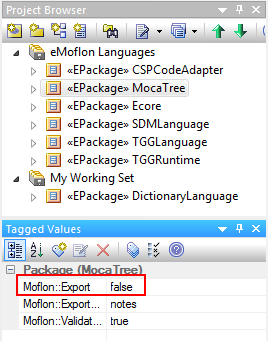
\includegraphics[width=0.4\textwidth]{ea_mocaTaggedValues}
  \caption{\texttt{MocaTree} is one of eMoflons' internal metamodels}
  \label{ea:mocaTagged}
\end{center}
\end{figure}

\end{itemize}

\vspace{-0.5cm}

If you inspect the tagged values\footnote{The ``Tagged Values'' window can be opened by going to ``View/Tagged Values'' or by hovering over the \texttt{Tagged
Values} tab immediately to the right of the project browser.} for these built-in languages, you'll notice that the \texttt{MocaTree} package has the
\texttt{Moflon::Export} value set to \texttt{false}. This ensures that the package is \emph{ignored} when exporting. As with all such standard metamodels (e.g.,
Ecore or our SDM metamodel) the \texttt{MocaTree} package in EA should be regarded as read-only, required only in the EA project so that SDMs/TGGs can refer to
the classes defined in the package.

\begin{itemize}

\item[$\blacktriangleright$] Despite \texttt{DictionaryLanguage} being contained in a different working set than \texttt{MocaTree}, the two
metamodels are contained within the same EA project (EAP) which means you are able to create a new TGG using them both. Add a new package to \texttt{My
Working Set} named \texttt{Dict\-ion\-ary\-Code\-Adap\-ter}.

\item[$\blacktriangleright$] Select the package and add a new TGG schema diagram as depicted in Fig.~\ref{ea:newTGGDiagram}. In the next dialogue window,
set the source project as \texttt{MocaTree}, and the target project as \texttt{Dict\-ion\-ary\-Lang\-uage}.

\begin{figure}[h!]
\begin{center}
  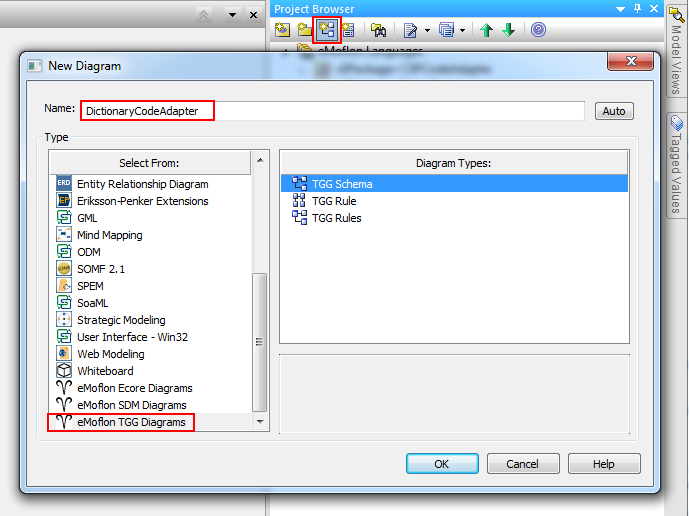
\includegraphics[width=0.9\textwidth]{ea_adapterTGGDiagram}
  \caption{Create a new TGG schema diagram}
  \label{ea:newTGGDiagram}
\end{center}
\end{figure}

\item[$\blacktriangleright$] For the moment, add a single correspondence type to the new diagram now active in the editor (the TGG \texttt{schema}) between
\texttt{Folder} and \texttt{Library}. Remember, you can get the classes by drag-and-dropping each element into the diagram, then quick-creating a new
\texttt{TGG Correspondence Type} between them.\footnote{For details on the correspondence metamodel and how to create types, refer to Part IV, Section 3.} Your diagram
should come to resemble Fig.~\ref{ea:firstCorrType}.

\vspace{0.5cm}

\begin{figure}[htpb]
\begin{center}
  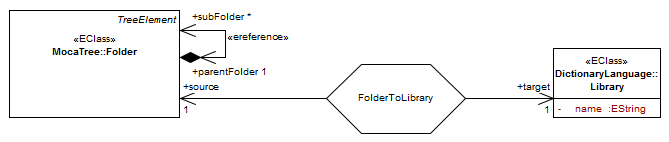
\includegraphics[width=\textwidth]{ea_firstAdapterCorrespondence}
  \caption{The first correspondence type for the transformation}
  \label{ea:firstCorrType}
\end{center}
\end{figure}

\newpage

\item[$\blacktriangleright$] Your complete project browser should now resemble Fig.~\ref{ea:TGGProjBrow}, where \texttt{Dict\-ion\-ary\-Code\-Adap\-ter} is now
explicitly listed as a \texttt{TGGSchemaPackage}.

\vspace{0.5cm}

\begin{figure}[htpb]
\begin{center}
  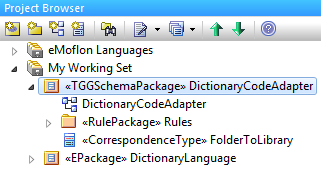
\includegraphics[width=0.5\textwidth]{ea_TGGProjectBrowser}
  \caption{A fully prepared TGG project}
  \label{ea:TGGProjBrow}
\end{center}
\end{figure}

\item[$\blacktriangleright$] Validate and export your file via the eMoflon control panel,\footnote{Activate via ``Extensions/Add-in Windows''} then switch
back to Eclipse and refresh the package explorer. A new \texttt{Dict\-ion\-ary\-Code\-Adap\-ter} project should appear in \texttt{My Working Set}.

\jumpSingle{subSec:setupParser}

\end{itemize}


\newpage
\hypertarget{M2TSettingUp tex}{}
\subsection{Initializing the project}
\texHeader

{\bf SELF:: update download so it includes a constraint file for \texttt{Dictionary}}
\begin{figure}[htbp]
\begin{center}
  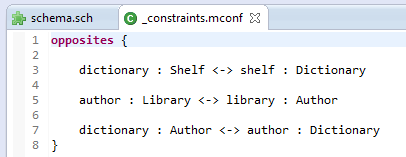
\includegraphics[width=0.7\textwidth]{eclipse_DOWNLOADUPDATE}
  \caption{SELF SELF}
\end{center}
\end{figure}

\begin{enumerate}

\item[$\blacktriangleright$] Your expanded \texttt{DictionaryLanguage} metamodel MOSL structure should resemble FIG. (starting point) You'll notice that it is
accessing the \emph{Moca} framework by importing the \texttt{MocaTree} in \texttt{\_imports.mconf}. (Explain, no screenshot?)

\item[$\blacktriangleright$] Right click on \texttt{MyWorkingSet} folder and create a new TGG. source: MocaTree. Target: DictionaryLanguage. FIG

\begin{figure}[htbp]
\begin{center}
  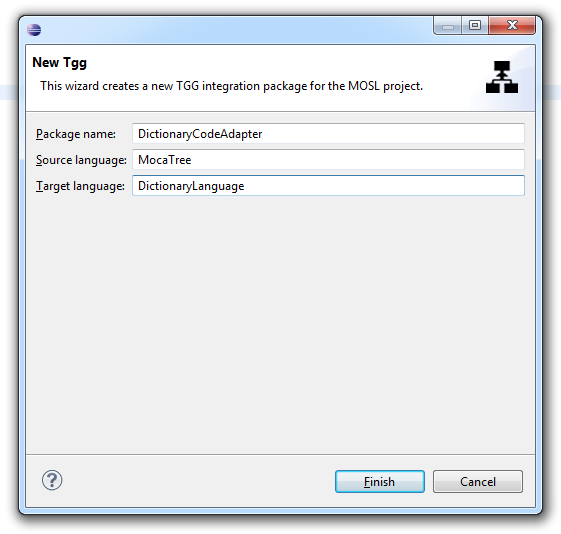
\includegraphics[width=0.9\textwidth]{eclipse_dictionaryCodeAdapterTGGProject}
  \caption{create tgg}
  \label{eclipse:newTGGProject}
\end{center}
\end{figure}


\item[$\blacktriangleright$] Before saving and building, initialize the correct generated code type by establishing the schema below (default is..)

\begin{figure}[htbp]
\begin{center}
  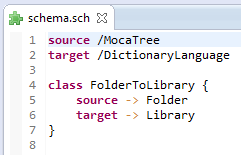
\includegraphics[width=0.5\textwidth]{eclipse_schemaStart}
  \caption{first rule}
  \label{eclipse:firstSchema}
\end{center}
\end{figure}

\item[$\blacktriangleright$] Save and build your project! Confirm a generated project was created in the \texttt{MyWorkingSet} node, and carry on!

\end{enumerate}


\newpage
\hypertarget{subSec:setupParser}{}
\subsection{Setting up the Parser}
\genHeader

\begin{itemize}

\item[$\blacktriangleright$] It should now resemble Fig.~\ref{eclipse:generatedAdapter}. Be sure to take a look at the \texttt{Moflon} and \texttt{Moca} library
nodes that reference jars for all required dependencies.

\begin{figure}[htpb]
\begin{center}
  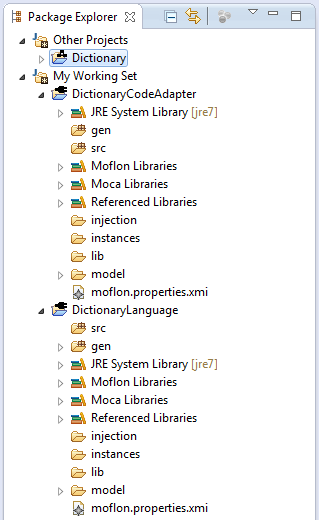
\includegraphics[width=0.4\textwidth]{eclipse_generatedAdapter}
  \caption{figureCaption}
  \label{eclipse:generatedAdapter}
\end{center}
\end{figure}

\item[$\blacktriangleright$] Right-click on \texttt{DictionaryCodeAdapter} and navigate to ``eMolfon/ Add Parser/Unparser'' (Fig~\ref{eclipse:contextParser}).

\begin{figure}[htpb]
\begin{center}
  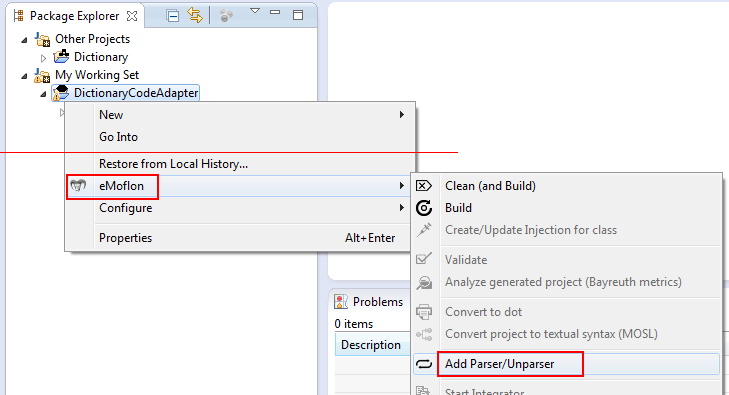
\includegraphics[width=0.9\textwidth]{eclipse_contextAddParserUnparser}
  \caption{figureCaption}
  \label{eclipse:contextParser}
\end{center}
\end{figure}

\item[$\blacktriangleright$] In the wizard dialogue (Fig~\ref{eclipse:wizardParser}), enter ``dictionary'' as the \texttt{File extension}, and make sure
the boxes \texttt{Create Parser} and \texttt{Create Unparser} with \texttt{ANTLR} are chosen as corresponding technology in both cases. Click \texttt{Finish} to
close.

\begin{figure}[htpb]
\begin{center}
  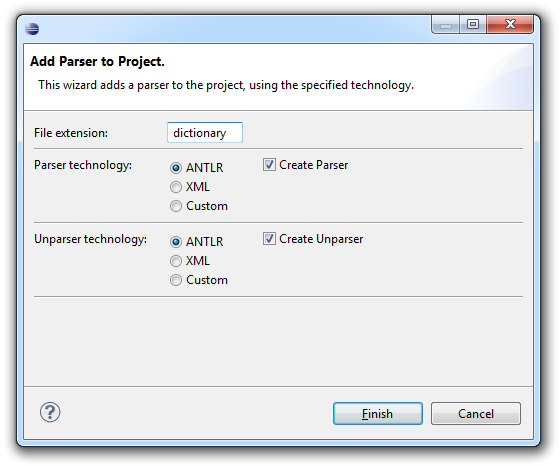
\includegraphics[width=0.8\textwidth]{eclipse_wizardParser}
  \caption{figureCaption}
  \label{eclipse:wizardParser}
\end{center}
\end{figure}

If everything has been installed and set up properly, parser and unparser stubs should be generated and \texttt{ANTLR} should automatically build the
corresponding Java code as depicted in Fig.~\ref{eclipse:generatedParser}.

\begin{figure}[htpb]
\begin{center}
  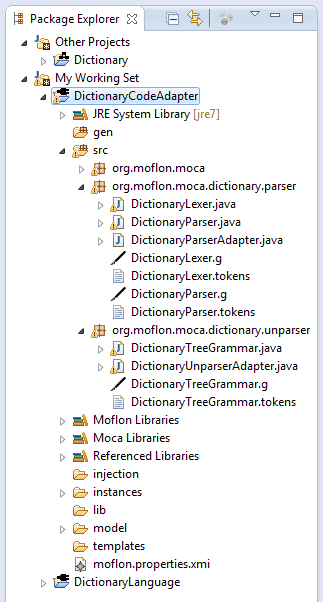
\includegraphics[width=0.4\textwidth]{eclipse_generatedParser}
  \caption{figureCaption}
  \label{eclipse:generatedParser}
\end{center}
\end{figure}

\end{itemize}

